

\tikzset{every picture/.style={line width=0.75pt}} %set default line width to 0.75pt        

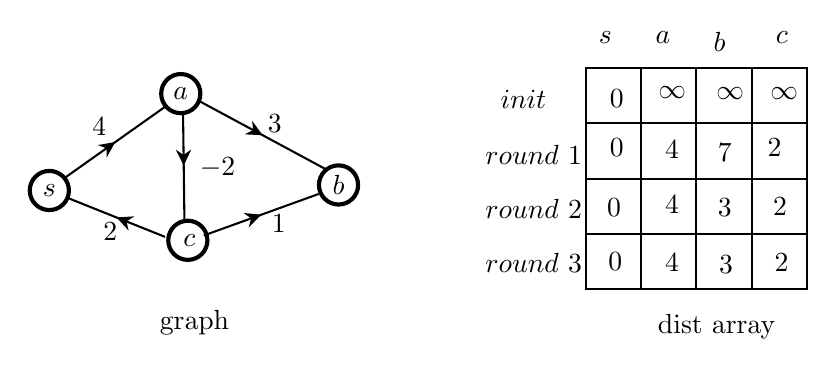
\begin{tikzpicture}[x=0.5pt,y=0.5pt,yscale=-1,xscale=1]
%uncomment if require: \path (0,244); %set diagram left start at 0, and has height of 244

%Straight Lines [id:da6460204159880261] 
\draw [color={rgb, 255:red, 0; green, 0; blue, 0 }  ,draw opacity=1 ][line width=0.75]    (44,115) -- (116,64) ;
\draw [shift={(80,89.5)}, rotate = 144.69] [fill={rgb, 255:red, 0; green, 0; blue, 0 }  ,fill opacity=1 ][line width=0.08]  [draw opacity=0] (11.61,-5.58) -- (0,0) -- (11.61,5.58) -- (7.71,0) -- cycle    ;
%Straight Lines [id:da6066395504516056] 
\draw [color={rgb, 255:red, 0; green, 0; blue, 0 }  ,draw opacity=1 ][line width=0.75]    (46,130) -- (116,158) ;
\draw [shift={(81,144)}, rotate = 21.8] [fill={rgb, 255:red, 0; green, 0; blue, 0 }  ,fill opacity=1 ][line width=0.08]  [draw opacity=0] (11.61,-5.58) -- (0,0) -- (11.61,5.58) -- (7.71,0) -- cycle    ;
%Straight Lines [id:da1865492813606927] 
\draw [color={rgb, 255:red, 0; green, 0; blue, 0 }  ,draw opacity=1 ][line width=0.75]    (227,127) -- (144,157) ;
\draw [shift={(185.5,142)}, rotate = 160.13] [fill={rgb, 255:red, 0; green, 0; blue, 0 }  ,fill opacity=1 ][line width=0.08]  [draw opacity=0] (11.61,-5.58) -- (0,0) -- (11.61,5.58) -- (7.71,0) -- cycle    ;
%Straight Lines [id:da7037921758898328] 
\draw [color={rgb, 255:red, 0; green, 0; blue, 0 }  ,draw opacity=1 ][line width=0.75]    (232,109) -- (141,60) ;
\draw [shift={(186.5,84.5)}, rotate = 208.3] [fill={rgb, 255:red, 0; green, 0; blue, 0 }  ,fill opacity=1 ][line width=0.08]  [draw opacity=0] (11.61,-5.58) -- (0,0) -- (11.61,5.58) -- (7.71,0) -- cycle    ;
%Straight Lines [id:da8291596598765129] 
\draw [color={rgb, 255:red, 0; green, 0; blue, 0 }  ,draw opacity=1 ][line width=0.75]    (129,68) -- (130,145) ;
\draw [shift={(129.5,106.5)}, rotate = 269.26] [fill={rgb, 255:red, 0; green, 0; blue, 0 }  ,fill opacity=1 ][line width=0.08]  [draw opacity=0] (11.61,-5.58) -- (0,0) -- (11.61,5.58) -- (7.71,0) -- cycle    ;
%Shape: Grid [id:dp9545383501398971] 
\draw  [draw opacity=0] (420,36) -- (580,36) -- (580,196) -- (420,196) -- cycle ; \draw   (460,36) -- (460,196)(500,36) -- (500,196)(540,36) -- (540,196) ; \draw   (420,76) -- (580,76)(420,116) -- (580,116)(420,156) -- (580,156) ; \draw   (420,36) -- (580,36) -- (580,196) -- (420,196) -- cycle ;

% Text Node
\draw (69.24,145.53) node [anchor=north west][inner sep=0.75pt]   [align=left] {$\displaystyle 2$};
% Text Node
\draw  [line width=1.5]   (32.38, 124.47) circle [x radius= 14.15, y radius= 14.15]   ;
\draw (32.38,124.47) node   [align=left] {$\displaystyle s$};
% Text Node
\draw  [line width=1.5]   (127.38, 54.47) circle [x radius= 14.15, y radius= 14.15]   ;
\draw (127.38,54.47) node   [align=left] {$\displaystyle a$};
% Text Node
\draw  [line width=1.5]   (132.48, 160.47) circle [x radius= 14.15, y radius= 14.15]   ;
\draw (126.98,160.47) node [anchor=west] [inner sep=0.75pt]   [align=left] {$\displaystyle c$};
% Text Node
\draw  [line width=1.5]   (241.38, 120.47) circle [x radius= 14.15, y radius= 14.15]   ;
\draw (241.38,120.47) node   [align=left] {$\displaystyle b$};
% Text Node
\draw (61.24,69.53) node [anchor=north west][inner sep=0.75pt]   [align=left] {$\displaystyle 4$};
% Text Node
\draw (188,67.47) node [anchor=north west][inner sep=0.75pt]   [align=left] {$\displaystyle 3$};
% Text Node
\draw (191,139.47) node [anchor=north west][inner sep=0.75pt]   [align=left] {$\displaystyle 1$};
% Text Node
\draw (139,98.47) node [anchor=north west][inner sep=0.75pt]   [align=left] {$\displaystyle -2$};
% Text Node
\draw (435.24,49.06) node [anchor=north west][inner sep=0.75pt]   [align=left] {$\displaystyle 0$};
% Text Node
\draw (345.24,89.23) node [anchor=north west][inner sep=0.75pt]   [align=left] {$\displaystyle round\ 1$};
% Text Node
\draw (427.24,7.56) node [anchor=north west][inner sep=0.75pt]   [align=left] {$\displaystyle s$};
% Text Node
\draw (468.24,7.56) node [anchor=north west][inner sep=0.75pt]   [align=left] {$\displaystyle a$};
% Text Node
\draw (510.24,7.56) node [anchor=north west][inner sep=0.75pt]   [align=left] {$\displaystyle b$};
% Text Node
\draw (555.24,7.56) node [anchor=north west][inner sep=0.75pt]   [align=left] {$\displaystyle c$};
% Text Node
\draw (470.24,47.06) node [anchor=north west][inner sep=0.75pt]   [align=left] {$\displaystyle \infty $};
% Text Node
\draw (512.24,48.06) node [anchor=north west][inner sep=0.75pt]   [align=left] {$\displaystyle \infty $};
% Text Node
\draw (551.24,48.06) node [anchor=north west][inner sep=0.75pt]   [align=left] {$\displaystyle \infty $};
% Text Node
\draw (356.24,50.06) node [anchor=north west][inner sep=0.75pt]   [align=left] {$\displaystyle init$};
% Text Node
\draw (549.24,85.06) node [anchor=north west][inner sep=0.75pt]   [align=left] {$\displaystyle 2$};
% Text Node
\draw (513.24,88.06) node [anchor=north west][inner sep=0.75pt]   [align=left] {$\displaystyle 7$};
% Text Node
\draw (435.24,85.06) node [anchor=north west][inner sep=0.75pt]   [align=left] {$\displaystyle 0$};
% Text Node
\draw (475.24,86.06) node [anchor=north west][inner sep=0.75pt]   [align=left] {$\displaystyle 4$};
% Text Node
\draw (475.24,126.06) node [anchor=north west][inner sep=0.75pt]   [align=left] {$\displaystyle 4$};
% Text Node
\draw (475.24,168.06) node [anchor=north west][inner sep=0.75pt]   [align=left] {$\displaystyle 4$};
% Text Node
\draw (433.24,128.06) node [anchor=north west][inner sep=0.75pt]   [align=left] {$\displaystyle 0$};
% Text Node
\draw (434.24,167.06) node [anchor=north west][inner sep=0.75pt]   [align=left] {$\displaystyle 0$};
% Text Node
\draw (513.24,128.06) node [anchor=north west][inner sep=0.75pt]   [align=left] {$\displaystyle 3$};
% Text Node
\draw (514.24,169.06) node [anchor=north west][inner sep=0.75pt]   [align=left] {$\displaystyle 3$};
% Text Node
\draw (554.24,168.06) node [anchor=north west][inner sep=0.75pt]   [align=left] {$\displaystyle 2$};
% Text Node
\draw (553.24,127.06) node [anchor=north west][inner sep=0.75pt]   [align=left] {$\displaystyle 2$};
% Text Node
\draw (345.24,128.4) node [anchor=north west][inner sep=0.75pt]   [align=left] {$\displaystyle round\ 2$};
% Text Node
\draw (345.24,167.56) node [anchor=north west][inner sep=0.75pt]   [align=left] {$\displaystyle round\ 3$};
% Text Node
\draw (110,209) node [anchor=north west][inner sep=0.75pt]   [align=left] {graph};
% Text Node
\draw (470,212) node [anchor=north west][inner sep=0.75pt]   [align=left] {dist array};


\end{tikzpicture}

